%SOP Template 
% Version 02 Added revision date
% Version 03 Added TOC and acknowledgements
%           New SOP3_alpha.cls


\documentclass[12pt]{../SOP3_alpha}\usepackage[]{graphicx}\usepackage[]{color}
%% maxwidth is the original width if it is less than linewidth
%% otherwise use linewidth (to make sure the graphics do not exceed the margin)
\makeatletter
\def\maxwidth{ %
  \ifdim\Gin@nat@width>\linewidth
    \linewidth
  \else
    \Gin@nat@width
  \fi
}
\makeatother

\definecolor{fgcolor}{rgb}{0.345, 0.345, 0.345}
\newcommand{\hlnum}[1]{\textcolor[rgb]{0.686,0.059,0.569}{#1}}%
\newcommand{\hlstr}[1]{\textcolor[rgb]{0.192,0.494,0.8}{#1}}%
\newcommand{\hlcom}[1]{\textcolor[rgb]{0.678,0.584,0.686}{\textit{#1}}}%
\newcommand{\hlopt}[1]{\textcolor[rgb]{0,0,0}{#1}}%
\newcommand{\hlstd}[1]{\textcolor[rgb]{0.345,0.345,0.345}{#1}}%
\newcommand{\hlkwa}[1]{\textcolor[rgb]{0.161,0.373,0.58}{\textbf{#1}}}%
\newcommand{\hlkwb}[1]{\textcolor[rgb]{0.69,0.353,0.396}{#1}}%
\newcommand{\hlkwc}[1]{\textcolor[rgb]{0.333,0.667,0.333}{#1}}%
\newcommand{\hlkwd}[1]{\textcolor[rgb]{0.737,0.353,0.396}{\textbf{#1}}}%
\let\hlipl\hlkwb

\usepackage{framed}
\makeatletter
\newenvironment{kframe}{%
 \def\at@end@of@kframe{}%
 \ifinner\ifhmode%
  \def\at@end@of@kframe{\end{minipage}}%
  \begin{minipage}{\columnwidth}%
 \fi\fi%
 \def\FrameCommand##1{\hskip\@totalleftmargin \hskip-\fboxsep
 \colorbox{shadecolor}{##1}\hskip-\fboxsep
     % There is no \\@totalrightmargin, so:
     \hskip-\linewidth \hskip-\@totalleftmargin \hskip\columnwidth}%
 \MakeFramed {\advance\hsize-\width
   \@totalleftmargin\z@ \linewidth\hsize
   \@setminipage}}%
 {\par\unskip\endMakeFramed%
 \at@end@of@kframe}
\makeatother

\definecolor{shadecolor}{rgb}{.97, .97, .97}
\definecolor{messagecolor}{rgb}{0, 0, 0}
\definecolor{warningcolor}{rgb}{1, 0, 1}
\definecolor{errorcolor}{rgb}{1, 0, 0}
\newenvironment{knitrout}{}{} % an empty environment to be redefined in TeX

\usepackage{alltt}
\usepackage[english]{babel}
\usepackage{blindtext}
\usepackage{lipsum}

%\documentclass{article}

%\documentclass[12pt]{~/github/SOPs/SOP_Template/SOP}

\title{Genomic DNA Extraction from Plants (Algae)}
\date{8/16/2016}
\author{Aparna Chintapalli}
\approved{Los Huertos}
\ReviseDate{\today}
\SOPno{24 v.01}
\IfFileExists{upquote.sty}{\usepackage{upquote}}{}
\begin{document}
%\SweaveOpts{concordance=TRUE}

\maketitle

\section{Scope and Application}

\NP The scope of this SOP is train researchers to become familiar with the steps and procedures involved in extracting genomic DNA from plant material, and in particular, algal species. With the use of equipment and materials provided in the Nucleospin Plant II Kit, DNA from plant samples can be successfully extracted by following proper protocol, safety precautions, and by paying close attention to the detailed instructions outlined in this handout, alongside the Professor. 

\NP The applications of this SOP are for various types of plant samples. As long as samples can be homogenized, this procedure for DNA extraction is applicable. 

\section{Summary of Method}

\NP Plant samples are homogenized by mechanical treatment or collected in a manner that does not require additional treatment (i.e. samples suspended in water/solvent). The DNA is then extracted with Lysis Buffers PL1 or PL2 containing chaotropic salts, denaturing agents, and detergents, which are used to break open cells and cell membrane structures so the DNA can be isolated. RNase A is included to remove RNA and allow photometric quantification of pure genomic DNA. Crude lysates from the samples are cleared by centrifugation and/or filtration using the Nucleospin Filters to remove polysacchardies, contaminations, and residual cellular debris. The clear flow-through that passes through filtration is mixed with binding buffer PC to create conditions for optimal binding of DNA to the silica membrane. After loading this mixture into the spin column, contaminants (proteins, RNA, metabolites, other PCR inhibitors) are washed away using Wash Buffers PW1 and PW2. The genomic DNA is finally eluted with low salt Elution Buffer PE or nuclease-free water to wash away unbound proteins.

\tableofcontents

\newpage

\section{Acknowledgements}

This SOP was originally written by Aparna Chintapalli after a SURP where she collected and extracted DNA from algae growing in the Santa Ana River.

\section{Definitions}

\NP All reagants and equipment are self explanatory in lab. 

\section{Interferences}

\NP The extraction process is supposed to isolate DNA from other cellular or organic materials. However, proteins and phenols...  

\NP When measuring the DNA yield, these compounds may interfere with the measurements and lead you to think that more DNA was extracted than actually was. See section QA/QC to learn how to measure these contaminants.

\NP Using the NanoDrop Spectrophotometer you can measuring the absorbance/transmission of light through a liquid to determine the concentration and purity of a specific substance, DNA in this case. In order to accurately measure the concentration of DNA based on its absorbance, you must know the wavelength of light at which it maximally absorbs. Nucleic acids (DNA and RNA) absorb at 260nm. Protein maximally absorbs at 280nm and the ratio of nucleic acid to protein (260/280) is generally used as an indicator of the purity of DNA samples.


\begin{description}
  \item[A260/A280 Ratio] A pure sample will produce a well defined peak(see Figure 1 below) at 260nm with the NanoDrop. Several factors, however, can influence the accuracy of the 260/280 and 260/230 ratios. Readings from very diluted samples will have very little difference between the absorbance at 260 and 280nm leading to inaccurate ratios.  The type(s) of protein present will also have an effect.  Absorbance in the UV range by proteins is primarily the result of aromatic ring structures. Phenol and other contaminants can also absorb at 280 nm and can affect the ratio calculation. Phenol absorbs with a peak at 270nm. \textbf{Nucleic acid preparations uncontaminated by phenol should have an 260/280 ratio of around 1.8. } The pH of the solution can also affect the 260/280 ratio, with acidic solutions having a lower ratio of up to 0.2–0.3 and alkaline solutions having an increased ratio by a similar amount.
  
  \item[A260/A230 Ratio] Pure RNA has an A260/A280 ratio of 2.0, therefore if a DNA sample has an 260/280 ratio of greater than 1.8 this could suggest RNA contamination. The 260/230 ratio is a secondary measure of nucleic acid purity. The ratio for pure samples is often higher than the respective 260/280 ratio values. Strong absorbance around 230nm can indicate that organic compounds or chaotropic salts are present in the purified DNA.  A ratio of 260nm to 230nm can help evaluate the level  of salt carryover in the purified DNA. The lower the ratio, the greater the amount of salt present. \textbf{As a guideline, the 260/230 ratio should be greater than 1.5, ideally close to 1.8.} (Compare 260/230 readings in Figures 1 and 2 Below) Urea, EDTA, carbohydrates and phenolate ions all have absorbance near 230nm. A reading at 320nm will indicate if there is turbidity in the solution, another indication of possible contamination.  
  
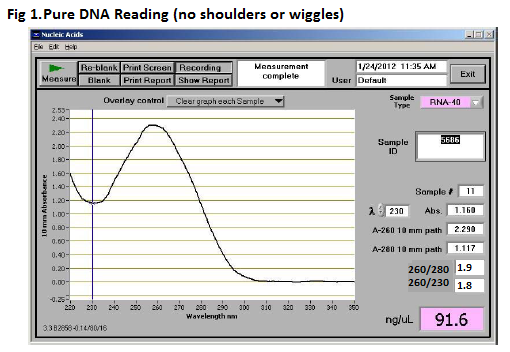
\includegraphics[scale=1]{NanoDropPure.png}

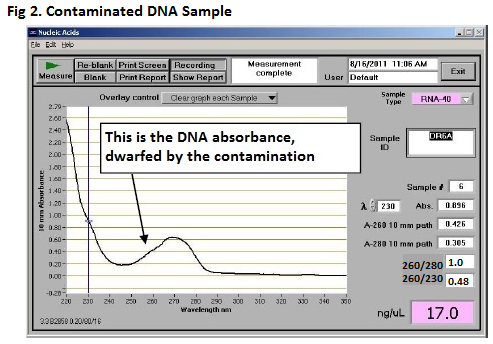
\includegraphics[scale=1]{NanoDropContaminated.png}

\end{description}

\section{Health and Safety}

\NP The risks involved with using this kit are mainly related to the chemicals that are in use. As listed below, safety precautions should be taken at all times, but especially when handling hazardous reagants. While following safety protocol, it is advised that the materials and equipment are kept organized to avoid contamination and thus yield good results. 

\NP CAUTION: PC and PW1 contain guanidine hydrochloride, ethanol, and isopropanol, beware of these chemicals coming into contact with the skin and especially the eyes. Also keep away from heat (highly flammable liquid and vapours).

\subsection{Safety and Personnel Protective Equipment}

\NP Always wear appropriate lab safety equipment, including safety goggles, lab coat, close-toed shoes, long pants, and gloves. 

\section{Personnel \& Training Responsibilities}

\NP Researchers training is required before the procedures in this method can be used... 

\NP Researchers using this SOP should be trained for the following SOPs:

\begin{itemize}
  \item SOP01 Laboratory Safety
  \item SOP02 Field Safety
  \item SOP03 Handling of Hazardous Materials
  \item SOP12 Using Hot Plates and Dry Baths
  \item SOP14 Microcentrifuge
  \item SOP09 Using Balances, Pippettes, and Glassware
  \item SOP16 Using Laboratory Refrigerators and Freezers
\end{itemize}


\section{Required Materials}

\subsection{Equipment}

\NP Bead homogenizer

\NP Microcentrifuge with rotor capable of reaching 4500g

\NP Pipettors 2 $\mu$L - 750 $\mu$L

\NP Vortex

\NP Thermal heating block or water bath for incubation

\NP Elution, mortar and pestle (if necessary for homogenization)

\subsection*{Reagents}

\NP 96-100\% Ethanol 

\subsection*{Consumables}

\NP DNA, RNA, and protein purification: Nucleospin Plant II Kit Red. 740770.50

\NP 1.5mL microcentrifuge tubes, 

\NP Disposable pipet tips


\section{Estimated Time}

\NP This procedure requires approximately 5-6 hours depending on the number of samples,and the time it takes to homogenize starting material and complete other preliminary steps. 

\section{Sample Collection, Preservation, and Storage}

\NP Store plant samples in freezer before homogenization.

\section{Procedure}

\subsection*{Preliminary Steps}
	 
\NP Mechanical treatment of plant samples can be done by grinding the material with a mortar and pestle in the presence of liquid nitrogen, without letting the sample thaw any time during this procedure. The mortar, pestle, and spatula to remove the sample must be precooled before grinding the sample into a fine powder. This step is not necessary for exeriments with algea.

\NP	Check that Wash Buffer PW2 and RNase A were prepared and stored appropriately according to the table found on page 14 of the user manual (made available by professor).

\NP Preheat 50 $\mu$L Elution Buffer PE in an Eppendorf tube to 65$^\circ$ C in the stainless steel Lab Armor machine at the back of the lab. Machine should be turned on 1 hour prior to use.

\NP The Nucleospin Plant II kits include two different lysis buffers; for optimal results, pair the buffer accordingly with your plant species by referring to the chart in the booklet or ask the Professor for further instruction. 


\subsection*{Homogenize the Sample}

\NP Homogenize up to 20 mg of dry weight plant sample via mechanical treatment (see prelim. prep). This is not necessary for experiments using algea. If sample is in water or other solvent, prepare up to 100 mg of wet weight by adding 20mL of the sample into a conical tube and centrifuging them. 

\NP Make sure to balance the tubes before loading into the centrifuge. Balance two tubes at a time by placing a plastic container on the balance with one tube in it. Then, tare the balance, and replace the tube with the other and add DI water to achieve same weight (within .1g ideally).

\NP Do this until all 4 tubes are balanced and place into the centrifuge with balanced pairs on opposite sides. Run the centrifuge at 4$^\circ$C for 20 min at 4000rpm.

\NP Unload the samples and remove most of the supernatant from each tube, leaving some of the liquid behind so the pellet at the bottom can be suspended and transferred easily. Using a wide tipped micropipettor, unload the samples into newly labeled 1.7mL Eppendorf tubes and place these into a smaller centrifuge for 1 min at 1000 rpm.


\subsection*{Cell Lysis}

\NP Into the prepared Eppendorf tubes, add 400$\mu$L Buffer PL1 and vortex the mixture thoroughly.NOTE: if the sample cannot be resuspended easily because it is soaking up too much buffer, add more PL1 (but increase RNase A proportionally).

\NP After vortexing, add 10$\mu$L RNase A solution (thawed) into each tube and mix thoroughly.

\NP Incubate the suspension for 10 min. at 65$^\circ$C. *For some plant material it might be advantageous to increase incubation time to 30 to 60 min. 

\subsection*{Filtration/Clarification of Crude Lysate}

\NP Place a Violet Ring Nucleospin Filter into a new 2mL Collection Tube and load lysate onto column for each sample. 

\NP Centrifuge these tubes for 2 min at 11,000 x g, and collect the clear flow-through (liquid at bottom) and discard the NucleoSpin filter above containing pellet/debris. If not all liquid passed through, repeat the centrifugation step.

\NP If a pellet is visible in the flow-through, transfer the clear supernatant to a new 1.5mL Eppendorf tube. 


\subsection*{Adjust DNA Binding Conditions}

\NP Add 450$\mu$L Buffer PC and mix thoroughly by pipetting up and down ($\sim$ 5 times) or by vortexing.


\subsection*{Bind DNA}

\NP Place a Green Ring Nucleospin Column into a new 2mL Collection Tube and load a maximum of 700$\mu$L of the sample.

\NP Centrifuge for 1 min at 11,000 x g and discard flow-through liquid, keeping the column in place above. 

\NP Because the maximum loading capacity of the column is 700$\mu$L, repeat the loading step for samples of higher volumes.

\subsection*{Wash and Dry Silica Membrane}

\NP 1st Wash: Add 400 $\mu$L Buffer PW1 to Green Column. Centrifuge for 1 min at 11,000 x g and discard flow-through.

\NP 2nd Wash: Add 700 $\mu$L Buffer PW2 to Green Column. Centrifuge for 1 min at 11,000 x g and discard flow-through.

\NP 3rd Wash: Add another 200$\mu$L Buffer PW2 to Green Column. Centrifuge for 2 min at 11,000 x g and discard flow-through. Run the samples again through the centrifuge for 1 min at 11,000 x g to complete a ``dry spin,'' ensuring that the wash buffer is completely removed and the silica membrane is dried completely. 

\subsection*{Elute DNA}

\NP Place the Green Column into a new 1.5mL Eppendorf tube and pipette 32$\mu$L Buffer PE (preheated at 65$^\circ$C) onto the membrane. 

\NP Incubate these tubes for 5 min at 65$^\circ$C. Then centrifuge for 1 min at 11,000 x g to elute the DNA.

\NP Repeat the previous step with another 50$\mu$L Buffer PE (65$^\circ$C) and elute into the same tubes, and run under centrifuge again.

\NP NOTE: Because Eppendorf tube caps do not close during this step, bend them at an angle before putting in the machine to avoid breaking them off. If they do however, simply transfer the liquid to new tubes.


\section{QA/QC}

\subsection*{Analysis of DNA Yield and Purity}

\NP You will now use the Nanodrop spectrophotometer to assess the purity of the DNA using UV radiation. 

\NP Open machine software and click on Nucleic Acid.

\NP Clean machine with Kimwipe before loading anything onto machine. 
\NP Pipette the Blank, whatever was used during elution (i.e. Elution Buffer), using a 2 $\mu$L pipettor onto the hydrophobic surface, creating a tiny bubble.

\NP Press Blank.

\NP Clean off surface, and repeate the previous step, but replace the elution buffer with each sample to be annalyzed.

\NP Load sample and press measure.

\NP Record the 260/280 and 260/230 ratios. They should be around 1.8-2.0 ideally. 

\section{Trouble Shooting}

\NP \textbf{NucleoSpin Filter or NucleoSpin Column is clogged.}
\begin{itemize}
  \item Centrifuge large amount of sample material before loading it into the filter.
  \item Make sure the cleared lysate is absolutely free of resuspended matter before loading it onto the NucleoSpin Plant Column.
 \item Increase centrifugation speed and time.
 \item Use more Lysis Buffer PL1 or PL2.
\end{itemize}

\NP \textbf{DNA is degraded.}
\begin{itemize}
  \item Sample is contaminated with DNAase.
  \item Centrifuge Speed was too high, causing shearing of the DNA.
\end{itemize}

\NP \textbf{DNA quality is low.}
\begin{itemize}
  \item Elution Buffer contains EDTA
  \item Salt or Ethanol carry-over. Make sure the last two wash steps were done with Wash Buffer PW2 and the membrane was dried according to the protocol.
\end{itemize}

\NP \textbf{DNA yield is low.}
\begin{itemize}
  \item Homogenization of plant material was not sufficient. 
  \item Suboptimal lysis buffer volume was used. Try PL1 and PL2 side by side to find the best detergent system to lyse your plant material. 
  \item Suboptimal lysis buffer volume was used. Cell Lysis might be insufficient and too much DNA might get lost during lysate clarification if dry material soaks up too much lysis buffer. Use more lysis buffer and increase the volume of Binding Buffer PC proportionally.
  \item Extraction of DNA from plant material during lysis was insufficient. Increase incubation time in lysis buffer (overnight).
  \item Suboptimal Elution. The DNA can either be eluted in higher volumes or by repeating the elution step up to three times. Incubate NucleoSpin Plant II Column with elution buffer at 65 degree Celsius for at least 5 minutes.
Also check the pH of the elusion buffer which should be in the range of pH 8.0-8.5.
\end{itemize}

\section{References}

\NP APHA, AWWA. WEF. (2012) Standard Methods for examination of water and wastewater. 22nd American Public Health Association (Eds.). Washington. 1360 pp. (2014).

\end{document}
